\documentclass[a4paper]{article}

\usepackage{xcolor}
\usepackage{fancyheadings}
\usepackage{graphicx}


\newcommand{\todo}[1]{\textcolor{red}{[#1]}}
\lhead{Open Universiteit}
\chead{IM0102, Design patterns}
\rhead{Eindopdracht}

\begin{document}
\pagestyle{fancy}

\section*{Studentgegevens}
\begin{description}
	\item [Cursuscode] IM0102
	\item Scenario 6: Meerdere slidesets
	\item [Naam] Gerwin van Dijken
	\item [Studentnummer] 852034983
	\item [Naam] Ewoud Westerbaan
	\item [Studentnummer] 852069942
\end{description}

\subsection*{Verklaring eigen werk}
Hierbij verklaren we, Gerwin van Dijken en Ewoud Westerbaan, dat we dit document zelf geschreven hebben.
\par
We bevestigen dat de tekst en het werk dat in dit document gepresenteerd wordt origineel is, en dat we geen gebruik hebben gemaakt van andere bronnen dan die welke in de tekst en in de referenties worden genoemd.

\section*{Aanpak}
Om te beginnen hebben we beiden individueel een probleemanalyse gemaakt. Dit zorgde ervoor dat we allebei voldoende inzicht hadden in de huidige applicatie en de gewenste aanpassing. Vervolgens hebben we de terminologie op elkaar afgestemd (Wat is een presentatie? Hoe noemen we een bepaalde volgorde van slides?). De basis voor de probleemanalyse was de huidige beschijving van de applicatie uit leereenheid 3 in combinatie met de source code. Vervolgens is deze uitgebreid met de concepten uit de scenario beschrijving.
\par
Vervolgens zijn we begonnen met het schetsen van het model; voornamelijk op conceptueel niveau. Dit gaf ons een praatplaat om te kunnen overleggen wat de relaties zijn. Vanuit de verantwoordelijkheden zijn we methodes gaan toevoegen en hebben we een gebruikerslaag `er op' gezet (view en controller). Daarna zijn we meer gaan specifieren wat de implementaties zijn van de concepten, inclusief de mogelijke uitbreiding zoals deze beschreven is in de opdrachtomschrijving. Gedurende het proces kwamen we beiden af en toe met heel andere ideeën (het iterator gedeelte `voelde' niet goed), maar dit is achteraf vooral gebruikt om het bestaande model te toetsen (als een soort advocaat van de duivel). Het ontwerp hebben we afgemaakt door het toevoegen van de factories, waarvoor we voor de gehele variability laag (dus implementaties van de Presentation, Slide en SlideItem met Item) één factory hadden. 
\par
Toen we beiden content waren met het ontwerp, zijn we de bestaande applicatie langzaam gaan omschrijven naar de nieuwe versie. Tijdens de implementatie hebben we kleine aanpassingen in het model gemaakt. Als voorbeeld is de factory voor de gehele variability laag geïmplementeerd als een aparte factory per commonality (dus de PresentationFactory, SlideFactory en SlideItemFactory) voor een duidelijkere splitsing van verantwoordelijkheden en om de applicatie in de toekomst eenvoudiger uit te kunnen breiden. De wijzigingen achteraf zijn niet op conceptueel niveau geweest.
\par
We hebben de applicatie afgemaakt door het toevoegen van JavaDoc en het implementeren van de functionaliteit om een presentatie via de gebruikers interface in te laden (wat noemenswaardig eenvoudig bleek met deze opzet).
\par
Het merendeel van de opdracht is om-en-om gedaan, omdat onze dagen die beschikbaar zijn voor studie verschillen.

\section{Probleemanalyse}
\subsection{Dingen}
\begin{description}
\item[Presenter] is een verzameling van presentaties, die allen gebruik maken van \'e\'en slides verzameling. E\'en van deze presentaties is actief. Bewerkingen (zoals volgende slide en volgende slide) worden op de actieve presentatie uitgevoerd.
\item[Presentatie] is de weergave van gespecificeerde slides in een vaste volgorde. Slides kunnen meerdere keren voorkomen. Een presentatie bevat een titel. Deze is altijd zichtbaar tijdens de weergave van de presentatie. In het programma kunnen meerdere presentaties beschikbaar zijn.
\item[Slide] is de weergave van een pagina op het scherm. Een slide heeft een titel, een nummer, slide items en heeft een bepaalde oppervlakte.
\item[Slide item] is een element op een slide. Slide items worden onder elkaar getoond en is van een bepaald type.
Een slide item wordt in een stijl gepresenteerd.
\item[Stijl] is een vorm van weergave van een slide item in termen van horizontale uitlijning, lettertype, kleur, en lettertypegrootte.
\end{description}

\subsection{Regels}
\begin{description}
\item[Presenter] bepaalt de huidige (actieve) presentatie.
\item[Presentatie] bepaalt de volgorde van de slides.
\item[Slide item] bepaalt de stijl van de weergave.
\item[Stijl] bepaalt hoe een slide item wordt weergegeven. 
\end{description}

\subsection{Verantwoordelijkheden}
\begin{description}
\item[Presenter] is verantwoordelijk voor het bijhouden en aansturen van de actieve presentatie. 
\item[Presentatie] is verantwoordelijk voor de correcte volgorde van de slides en het beschikbaar stellen hiervan. 
\item[Slide] kan zijn titel tonen en de slide items schalen en onder elkaar laten tekenen.
\item[Slide item] kan zichzelf tekenen.
\end{description}
Overige verantwoordelijkheden die in de applicatie verwerkt moet worden:
\begin{description}
\item[Inlezen] van een XML bestand waarin de presentaties opgeslagen zijn. Uit dit bestand moet de slides verzameling en presentaties opgebouwd worden.
\item[Laten zien] van een gebruikers interface. Een gebruiker moet een presentatie kunnen kiezen, de presentaties kunnen bekijken en er doorheen kunnen navigeren.
\end{description}

\subsection{Aannames}
\begin{description}
\item[Niet opslaan] De bestaande applicatie bevat een hele sumiere opslag functionaliteit. De basis van de applicatie is dat het een alleen-lezen applicatie is (functionaliteit als het aanpassen van presentaties zit er niet in). Om deze reden hebben we geen opslag functionaliteit in de nieuwe versie zitten. Openen heeft wel toegevoegde waarde, dus deze zullen we wel implementeren.
\item[Niet wijzigen] De huidige applicatie bevat geen functionaliteit om wijzigingen door te voeren in presentaties. Wij zullen dit ook niet implementeren.
\item[Niet nieuw] Om dezelfde als dat we geen opslag functionaliteit aanbieden, laten we ook het aanmaken van een nieuwe presentatie achterwegen.
\end{description}

\section{Ontwerp}
\begin{description}
\item[Presenter] is verantwoordelijk voor de omgang van meerdere presentaties en het bijhouden wat de actieve presentatie is. Het biedt afnemers de mogelijkheid om een presentatie te kiezen.
\item[Presentation] is verantwoordelijk voor de correcte volgorde van de slides, het beschikbaar stellen hiervan en afnemers laten weten dat de slide beschikbaar is. Het biedt mogelijkheden om door slides te navigeren.
\item[Slide] is verantwoordelijk voor het tekenen van zichzelf.
\item[SlideItem] Zorg dragen voor het tekenen van items.
\item[Item] is verantwoordelijk voor het tekenen van zichzelf.
\item[Reader] is verantwoordelijk voor het laden van presentaties.
\end{description}
Om te kunnen reageren op wijzigingen van het model, zijn er twee observers gespecificeerd:
\begin{description}
\item[PresentationObserver] verantwoordelijk voor het reageren op wijziging van de presentatie. Bijvoorbeeld het veranderen van een presentatie.
\item[SlideObserver] verantwoordelijk voor reageren op het wijzigen van de aangeboden slide (dat er een andere slide ter beschikking wordt gesteld).
\end{description}

\section{Keuzen}
\begin{description}
\item[Model-View-Controller] als architectuur ontwerp. Het model is verantwoordelijk voor het kenbaar maken van wijzigingen. Dit wordt gedaan door het Observer patroon twee keer toe te passen.
\item[PresentationObserver] In deze versie van de applicatie is de toevoeging dat er met andere presentaties (volgorde van slides) gewerkt moet kunnen worden. Om andere objecten te laten weten dat de presentatie gewijzigd is, hebben we een PresentationObserver gemaakt. Aan de observers wordt de nieuw actieve Presentation gegeven.
\begin{itemize}
\item Subject: Presenter
\item Observer: PresentationObserver
\end{itemize}
\item[SlideObserver] Voor het kenbaar maken dat een andere slide getoond moet worden, hebben we gekozen voor het observer pattern. De reden is dat in de toekomst mogelijk andere observers ook acties moeten uitvoeren op het moment dat een andere slide getoond wordt. Te denken is aan een presentatorscherm waar opmerkingen op getoond worden. Aan de Observers wordt de nieuw actieve Slide gegeven.
\begin{itemize}
\item Subject: Presenter
\item Observer: SlideObserver
\end{itemize}
Omdat bij het selecteren van een andere presentatie we niet willen dat alle (slide)observers zich weer opnieuw moeten aanmelden, hebben we er voor gekozen om het aansturen van de presentatie via de Presenter te laten verlopen. De huidige presentatie is als het ware verstopt (encapsulated) in de Presenter.
\item[Iterator] Voor het aanbieden van slides aan de afnemer hebben we gekozen voor een (soort van) iterator patroon. De afnemers, alle SlideObservers, moeten de beschikking hebben over de objecten (Slides). Toch is dit geen zuivere Iterator in die zin dat de afnemende objecten niet vragen aan de Aggregate (Presenter) om een specifieke Iterator (Presentation) en hier methodes op aanroepen. In deze implementatie houdt de aggregate (de Presenter in ons geval) zelf bij wat de actieve iterator is, dit is immers zijn verantwoordelijkheid. Een actie als next() en previous() zal de Presenter op de actieve Iterator (Presentation) doen. Omdat de Presenter de Presentations gebruikt, creeërt de Presenter deze Presentations dus niet (in tegenstelling tot een klassieke iterator patroon), maar wordt dit gedaan door een factory (scheiding van creatie en gebruik).
\begin{itemize}
\item Aggregator: Presenter
\item Iterator: Presentation
\item ConcreteAggregator: PresentationManager
\item ConcreteIterator: SlideSequence
\end{itemize}

\item[Strategy] De SlideItem heeft een Item en een Style. De SlideItem geeft de Style aan de Item om deze zichzelf te tekenen. De implementatie van het tekenen met een gegeven stijl kan anders zijn voor de verschillende type items.
\begin{itemize}
\item Strategy: Item
\item ConcreteStrategies: TextItem, BitmapItem
\item Context: SlideItem
\end{itemize}

\item[Factory] Voor het aanmaken van objecten (via \texttt{new})  zijn er diverse Factory classes gemaakt. Dit zorgt er voor dat het gebruik en het aanmaken van objecten gescheiden is, en de applicatie volledig (met uitzondering van de factories) tegen interfaces aan programmeert. 

\item[Singleton] Om de factories voor de gehele applicatie toegankelijk te maken, zijn deze als Singleton geimplementeerd. De factory objecten worden dus alleen aangemaakt bij het eerste gebruik; latere verwijzingen werken met dezelfde (unieke) instanties.

\end{description}
\subsection{Toekomstige veranderingen}
\begin{description}
\item[Bepaalde delen laten zien] Het laten zien van bepaalde delen van een slide is gegeven als een mogelijke verandering. Dit is te implementeren door een nieuwe concrete klasse te definiëren die de Slide interface implementeert. Door deze klasse een associatie te geven naar de SlideDeckSlide kan de klasse de SlideItems benaderen. De implementatie van de draw() methode hoeft dan alleen deze specifieke SlideItems op te halen. De SlideFactory zal wel aangepast moeten worden om de nieuwe implementatie als Slide terug te kunnen geven. Zo ook de Reader objecten omdat dit ook een wijziging is in hoe de presentaties zijn opgeslagen. Zie Figure \ref{fig:mogelijkeuitbreiding}, de concrete klasse is hier PresentationSlide genoemd.
\begin{figure}[htbp]
\caption{Mogelijke uitbreiding (specificatie)}
\centering
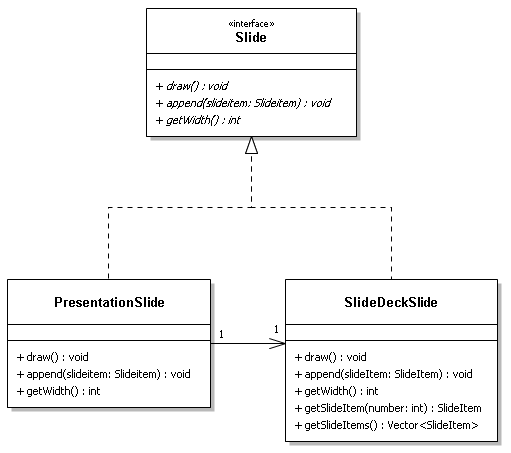
\includegraphics[width=0.75\textwidth]{MogelijkeUitbreiding.PNG}
\label{fig:mogelijkeuitbreiding}
\end{figure}

\textbf{Gerwin: "List\textless int \textgreater slideItemIndices wijzigen in List \textless SlideItem \textgreater slideItems...???"}

\item[Meerdere views] Zoals al aangegeven bij de observer pattern, is het mogelijk om bijvoorbeeld een aparte presentator view te maken waar opmerkingen op te zien zijn.
\item[Andere type items] Het is mogelijk om andere type items te tonen op een slide, door een nieuwe concrete klasse te maken die de Item interface implementeerd (naast de huidige TextItem en BitmapItem).
\item[Andere type bronnen] Een mogelijkheid voor uitbreiding is om presentaties ook te kunnen laden van andere type bronnen, bijvoorbeeld een JSON-file of een database. De ReaderFactory kan de benodige implementatie van Reader teruggeven en deze implementatie de benodige informatie geven via de constructor. Een voorbeeld is dat de DemoReader geen input nodig heeft, maar de XMLReader wel.  De load() functie in de Reader interface is zonder argumenten.
\end{description}

\section{Sourcecode}
Naast onderstaande beschrijving bevat de sourcecode commentaar en beschrijvende tekst in JavaDoc formaat.

\begin{description}
\item[Start van de applicatie] Het programma JabberPoint start met (in de main-methode in class JabberPoint) het aanmaken van hoofdobject Presenter via de PresenterFactory. Deze factory bepaalt welke concrete class gebruikt wordt als Presenter; de applicatie zelf weet dat niet, die kent alleen de interface ‘Presenter’.
Nadat de Presenter aangemaakt is, wordt er een SlideViewerFrame aangemaakt, waarin (via een SlideViewerComponent) een presentatie slide getoond kan worden. Deze SlideViewerFrame meldt zich aan bij de Presenter als PresentationObserver, waardoor deze bij het switchen naar een ander presentatie de juiste titel kan tonen. De SlideViewerComponent meldt zich ook bij de Presenter aan, maar dan als SlideObserver; de SlideViewerComponent moet namelijk bij een slide-switch de nieuwe slide tonen.
Zodra het frame (en component) aangemaakt zijn, wordt vanuit de main-methode een demo presentatie aangemaakt of een presentatie vanuit een bestand ingelezen (als er een bestandsnaam ingesteld is als programma argument). Van deze presentatie wordt de eerste slide geselecteerd.
De main heeft zijn werk gedaan; wat rest is een Presenter-object die een huidige/actieve presentatie bevat, en een view die de huidige slide daarvan toont.
\item[Controllers]
Omdat de applicatie natuurlijk door een gebruiker aangestuurd moet kunnen worden, zijn er een tweetal controllers op het SlideViewerFrame actief: een KeyController en een MenuController. \todo{de controllers zijn actief op een view???}  De KeyController handelt specifieke keyboard toetsen af, zoals PageUp/PageDown voor respectievelijk vorige en volgende slide van de huidige presentatie. De MenuController handelt de menuitems af, waaronder het selecteren van een andere presentatie, het inlezen van een nieuwe presentaties en het springen naar een specifieke slide (via een ingetoetst slide nummer). Beide controllers communiceren alleen met het Presenter object. De Presenter zal presentatie-handelingen (zoals next/previous slide) doorsluisen \todo{spreektaal? `doorgeven' msschien beter?} naar de actieve presentatie.
\item[Inlezen van presentaties]
Het inlezen van presentaties gaat via de Presenter. Momenteel kan een (hardcoded) demo presentatie aangemaakt worden en kunnen er presentaties via een xml-bestand worden ingelezen. Het inlezen van presentaties via een xml-bestand verloopt via een ReaderFactory. Deze factory bepaalt aan de hand van de extensie (bv “.xml”) welke concrete reader wordt ingezet voor het laden van een presentatie. De enige opties zijn momenteel een DemoReader en een XMLReader. Deze laatste reader maakt een lijst met Slide-objecten aan, en maakt vervolgens presentaties aan die elk verwijzen naar de aangemaakte Slide-objecten. Op deze manier kunnen er meerdere presentaties (variaties) gemaakt worden die gebruik maken van dezelfde slide, waarbij elke presentatie een andere slide-volgorde kan toepassen, slides kan overslaan of herhalen. Vanuit elke presentatie wordt verwezen naar de aangemaakte slide-objecten; deze worden dus niet gedupliceerd.
Na het inlezen van nieuwe presentaties wordt de eerste presentatie geselecteerd. De Presenter zal bij elke presentatie-switch een notificatie uitsturen naar alle PresentationObservers, waaronder de eerder genoemde SlideViewerFrame. Verder zal de Presenter bij elke presentatie-switch de eerste slide van deze presentatie selecteren; hierbij wordt een notificatie uitgestuurd naar alle SlideObservers, waaronder de eerder genoemde SlideViewerComponent. Informatie over de nieuwe presentatie en (eerste) slide zal dus meteen door de views worden getoond.
\item[Tonen van een presentatie slide]
Het tonen van een presentatie is niets anders dan het tonen van de huidige slide, wat op zijn beurt niets anders is dan het tonen van al zijn slide-items (de titel van de slide wordt als eerste slide-item getoond, waardoor deze steeds bovenaan op de slide staat). Bij het tekenen van een slide-item wordt een schaalfactor meegegeven; deze factor is de verhouding van de huidige window en de oorspronkelijk grootte. Als de applicatie-window door de gebruiker verkleind/vergroot wordt, dan zullen de items met dezelfde verhouding getekend worden.
De items worden altijd onder elkaar getoond, waarbij de verticale afstand door de hoogte van een “boudingbox” wordt bepaald. Elk specifieke item (tekst, plaatje, …) kan deze boundingbox bepalen. De hoogte is niet alleen afhankelijk van datgene wat getoond wordt (tekst, plaatje, …), maar ook van de ingestelde stijl. Elk item bevat een stijl dat gebruikt wordt bij het tonen, waardoor o.a. de (horizontale) inspringing en (verticale) regelafstand ingesteld kan worden.
\end{description}

\subsection{Packages}
De sourcecode files zijn onderverdeeld in verschillende packages.
\begin{description}
\item[controller] bevat de controllers KeyController en MenuController.
\item[views] bevat de classes SlideViewerComponent (een JComponent) en SlideViewerFrame (een JFrame).
\item[model] bevat diverse model classes zoals Presenter, Presentation, Slide en SlideItem.
\item[observer] bevat de interfaces PresentationObserver en SlideObserver.
\item[reader] bevat de (interface) Reader en (concrete classes) DemoReader en XMLReader.
\item[factory] bevat de classes PresentationFactory, PresenterFactory, ReaderFactory, SlideFactory, SlideItemFactory en StyleFactory. Elke factory is als een Singleton geïmplementeerd.
\end{description}
De class Jabberpoint, waar de applicatie start staat direct in de root van de applicatie.

\end{document}
